\section{Classification}
The use case of this article, is to help third-party evaluators find usability problems in a usability test.
In a usability test, the goal is to find usability problems, in other words the usability problems are unknown prior discovery. This is relevant for a classifier, because different strategies exist for different types of data. In this case, we do not have ``usability-problem labelled'' data on which we can train the classifier to detect problems which are similar. Because of this, a classifier which can detect anomalies from a training set which does not contain anomalies is required.
Additionally a usability test is generally considered to have mostly ``normal usage'' and only a portion of the entire system will contain usability problems. In other words, the majority of the physiological data collected can be considered expected normal responses, and only the portions of the system where a usability problem is present will result in anomalies.
This type of data fits the scope of novelty detection\cite{noveltyDetection}.

There are many different methods which can be applied when working with novelty detection\cite{noveltyDetection}, and choosing the right one is not a trivial task.
The different methods can be divided into five subgroups: probabilistic, distance based, domain based, reconstruction based, and information theoretic.
Manevitz et al.~\cite{oneClassSVM} showed that a \textit{one-class} SVM achieved on average better results than other classification techniques as neural networks, naive bayes, nearest neighbor and prototype over a series of dataset.
This paper use a one-class SVM as the classifier.
The goal of the classification in this paper is to explore the one-class SVM's behaviour when used to detect usability problems.

\subsection{One-class SVM}
The one-class SVM is a domain based algorithm used for novelty detection, meaning it creates a boundry given its training data.
Unseen data to be classified is then labelled as a normality or anomaly depending on its position relative to the boundry.
This can be seen on Figure \ref{[FIGURE] OneClass SVM}.

\begin{figure}
    \centering
  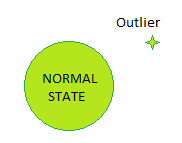
\includegraphics[width=0.75\columnwidth]{graphics/oneclass-svm.png}
    \caption{The circle ``Normal State'' is the area of which any data considered has to be inside, if it's ``normal''. The outlier will be labelled as an anomaly i.e. usability error for the user because it does not fit within the model/area of normalities. }
    \label{[FIGURE] OneClass SVM}
\end{figure}

Since the one-class SVM is sensitive\cite{oneClassSVM} to its parameter settings, a grid search is performed on them. The $Gamma = \{2^{-14},..,2^2\}$ value is, together with the Sigmoid and RBF kernel values. This is done to find the optimal settings where ``Nu parameter'' is kept at 0.05.
The library LibSVMSharp\cite{libsvmsharp} is used. It is a C\# wrapper for LibSVM\cite{libsvm} which is a widely used SVM library which also contains a one-class SVM implementation. The main reason LibSVMSharp is used over the native LibSVM is because it can be used in conjunction with the developed software used to collect and handle data, which is written in C\#.

\subsection{Prediction \& Scoring}
We create a one-class SVM for each of the sensors, where each of the SVMs trains on the data from the first two tasks, which contain no usability errors e.g. no anomalies. The model created can then be used to predict on the remaining data which has been collected when usability errors were present.
A one-class SVM will label a given data point with a binary answer. ``1'' for a normality, and ``-1'' for an anomaly.
This results in a collection of data points labeled as either a normality or an anomaly.

To decide whether an anomaly correctly corresponds to a usability error, that is it has \textit{hit} a usability error, some assumptions have to be made. 
Given tasks' events in the experiment is grouped into ``instant error feedback'' and ``non-instant error feedback'', two strategies has to be used. 
For instant error feedback the usability error is said to have been experienced by the participant at the specific time the error happened. In other words, if the error happens at time $t$, then the participant is also exposed to the stimuli / frustrating event at time $t$.
For non-instant error feedback the usability error is said to have been experienced during the timespan of the first event to the last event which are related to the task. This is illustrated in Figure X.X. \todo{Make figure of this}

When an anomaly is found an area of 2.5 seconds prior and after the anomaly is marked to create a point of interest. 
A point of interest spans 5 seconds in order to create a relevant time-snippet for a third-party evaluator to look at, rather than having a 1 millisecond span of time.

To evaluate if an event is correctly found by the machine the two types of events will be considered again.
The events which contain instant feedback is classified as a hit, if the points of interest covers the time at which the event happens.
For events which do not contain instant feedback the event will be hit, if the point of interest hits inside the area of the collection of events. Both of these examples is illustrated in Figure x.x. \todo{Make Figure}

Two scoring functions are used to optimize the gamma value in the line search. The first function is defined as: 
\[CovScore = \frac{2 \times EventsHitRate \times 1-FalseCoverRate}{EventsHitRate + FalseCoverRate}\]
Where \textit{EventHitRate}(EHR) describes how many of the existing events has been hit by an anomaly e.g. $EHR = \frac{DifferentEventsHit}{TotalNumberOfEvents}$, and \textit{FalseCoverRate}(FCR) is the rate of which the area outside events that has been covered e.g $FCR = \frac{NonEventAreaCovered}{TotalNonEventArea}$. 
The scoring function is the harmonic mean of EHR and FCR which is a kind of averaging of the two rates.
A low score from this function will the machines which have a low EHR and/or high FCR would make the numerator approach zero, while having a high EHR and low FCR will make the function approach 1 which is the ideal result.
Meaning this function rewards hit as many different events higher than hitting the same multiple times, while also considering the rate of FCR.
The second function is defined as: 
\[HitScore = \frac{2 \times EventsHitRate \times Presicion}{EventsHitRate + Precision}\]
Where \textit{Precision} is the rate of which the anomalies found by the SVM hits an event e.g. $precision = \frac{hits}{hits+misses}$. 
As with the first scoring function the second scoring function is a harmonic mean but with EHR and precision.
Meaning the function rewards spreading of the answers while having a high true positive rate on its guesses.


Since the Nu parameter indirectly dictates how much of the training data that should be inside the boundry of the ``normal state'', an examination of the Nu parameter impact on the results is conducted.\todo{Kan ikke lide den her sætning men har skrevet den anywho}
This is done using a line search, locking all the parameters except the $Nu = \{0.01, 0.02,.., 1\}$ and analyzing the difference in the result. 
